\chapter{Sample characterization}

There are two dimensions to characterize the quality of a sample. Its optical properties must include narrow linewidths, to identify different features of the spectrum and it has to be gate-tunable, which means the contact of \tmdg flake to the electrode as well as the backgate have to function and the \sio layer has to sustain enough voltage to tune in and out of neutral and charged regimes.

\section{Optical setup}

\begin{figure}
	\centering
	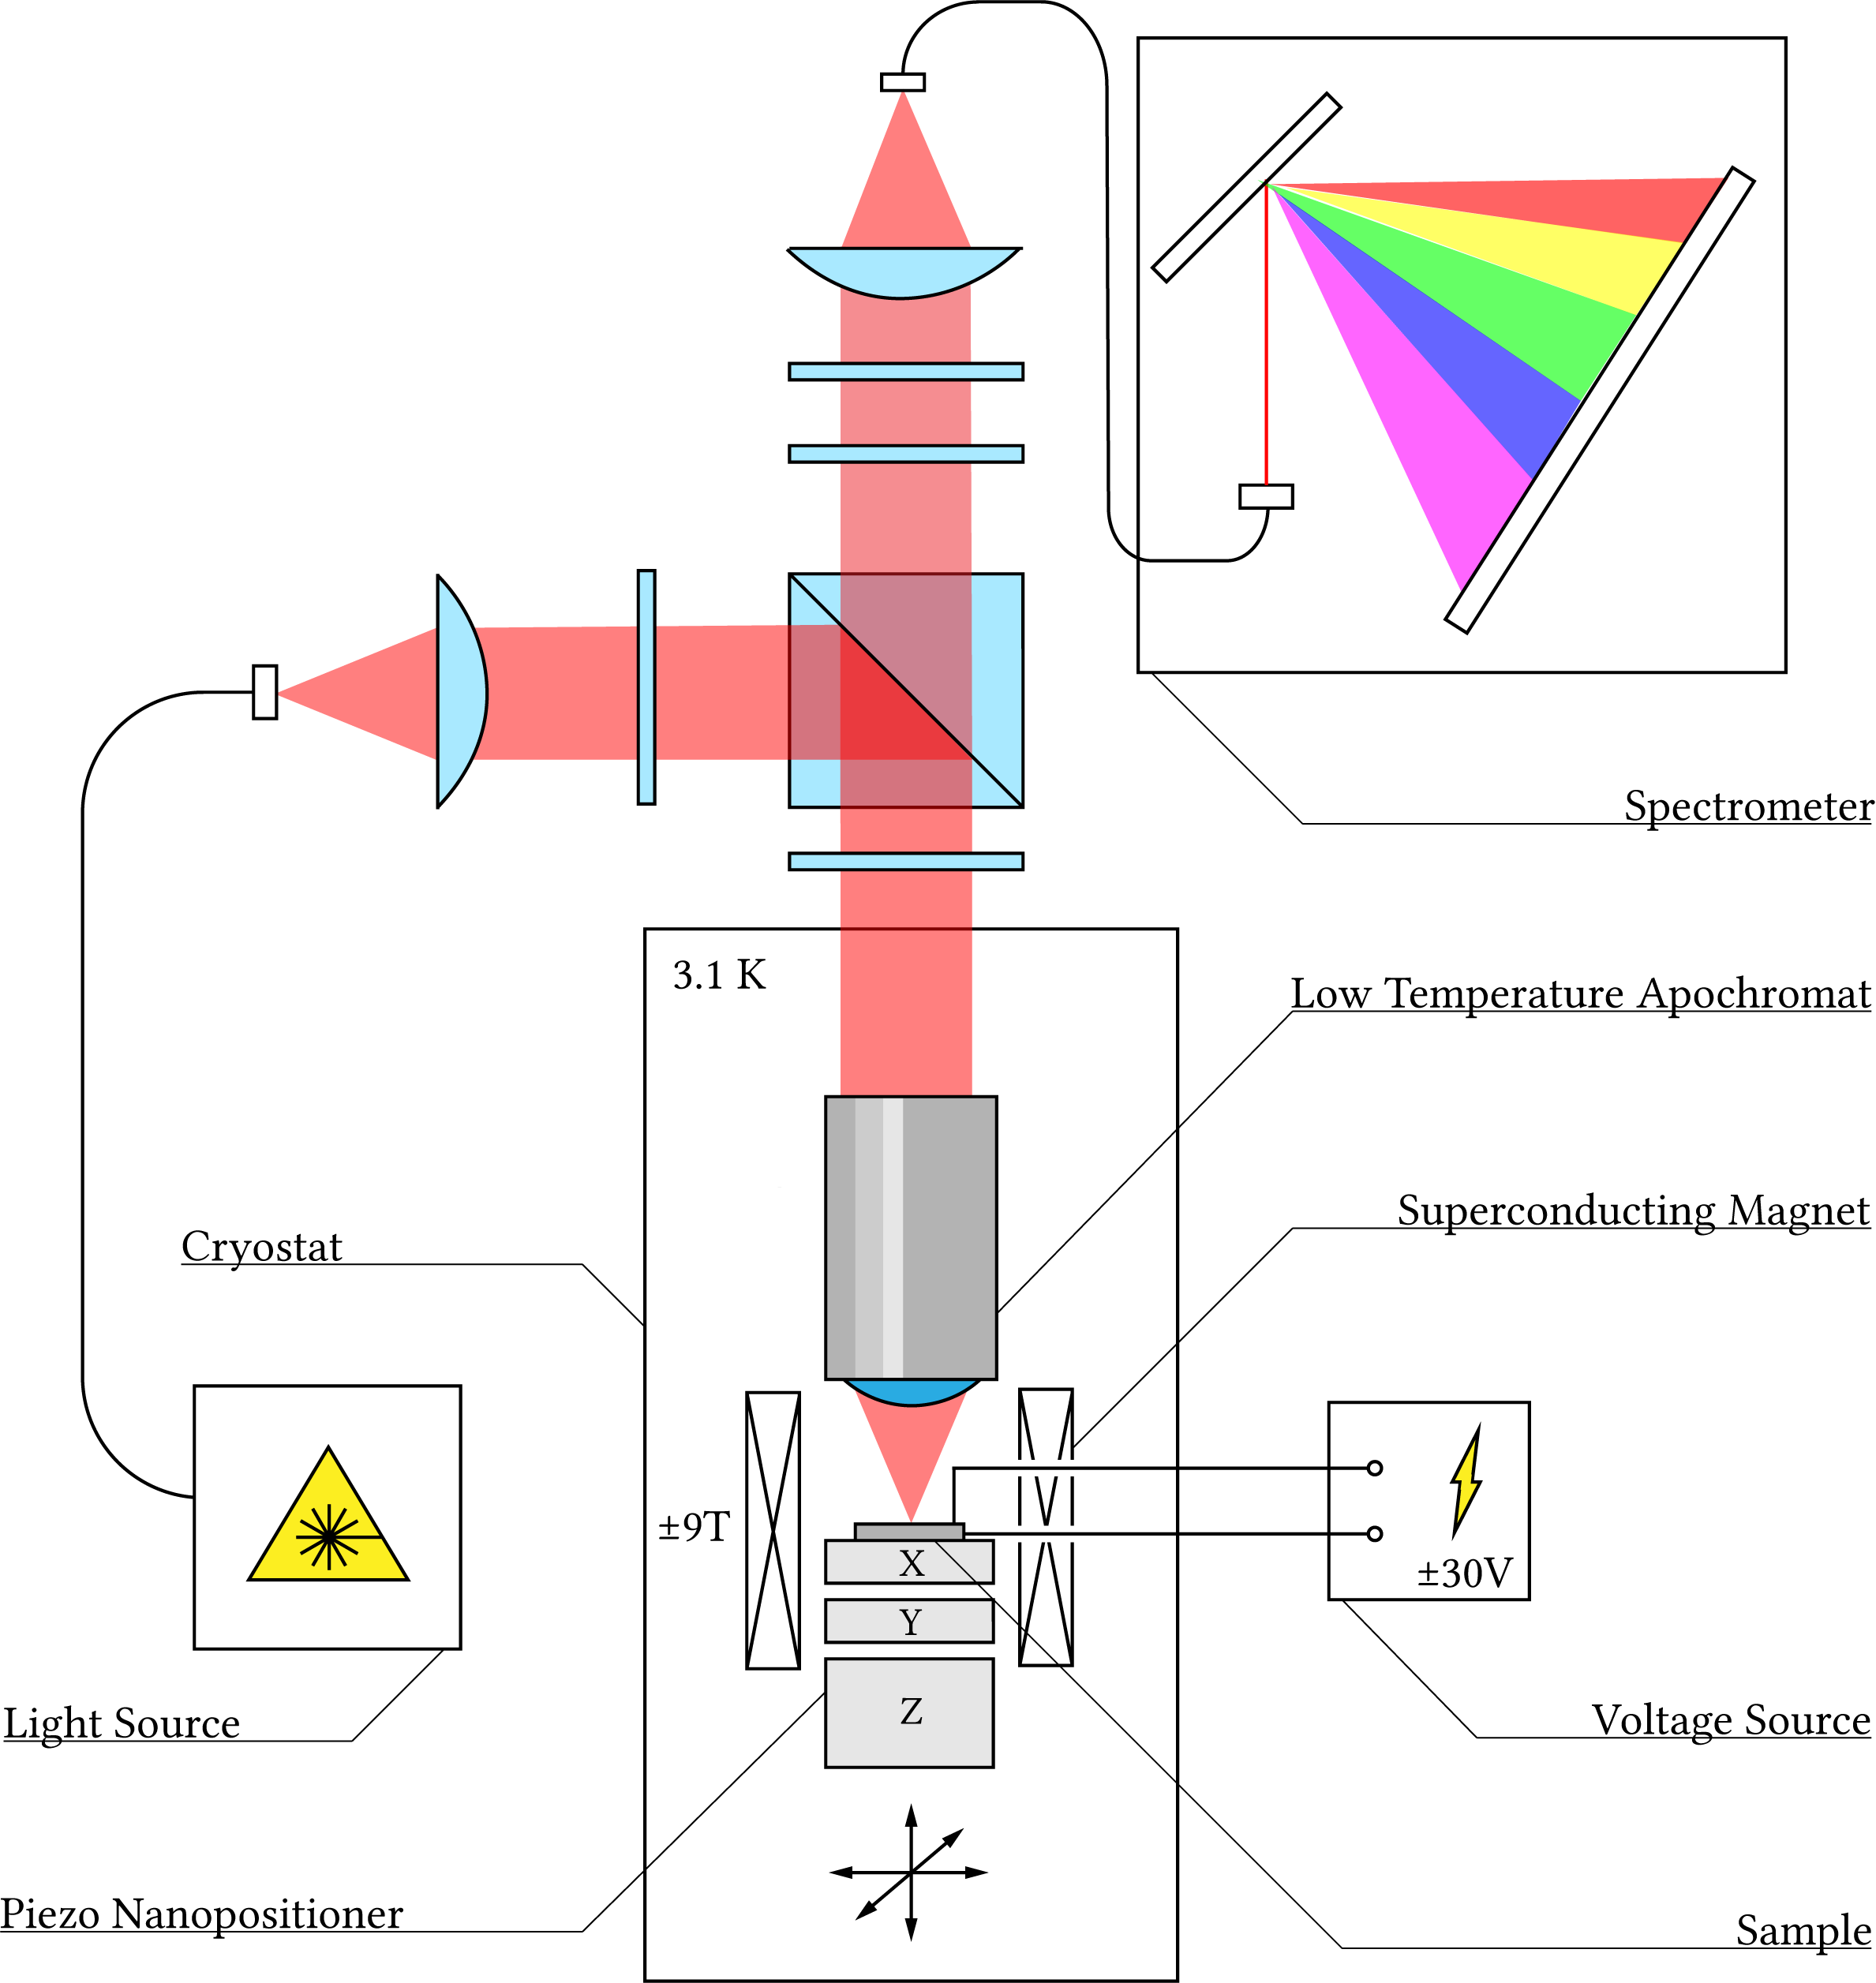
\includegraphics[width=.8\textwidth]{OptischerAufbau.png}
	\caption{Optical setup for confocal spectroscopy: Light from a \textbf{laser}-source is guided to the setup in a single mode opical fibre and collimated. To cut off raman-modes, that are created in the fibre a \textbf{shortpass} filter is installed behind the collimator. A \textbf{linear polarizer} defines a polarization axis. A \textbf{beam-sampler} is reflecting the excitation beam into a \textbf{low temperature apochromat}, whose focus lies on the sample, with a spotsize of \textasciitilde\- 0.5\mu m. The sample is mounted on a \textbf{piezo nanopositioner}, that is placed inside a \textbf{cryostat} at a temperature of up to 3.1 K or in a container of liquid helium at 4.2 K. The cryostat is equipped with a \textbf{superconducting magnet} that can supply a homogenious magnetic field up to 9T. The sample electrodes are connected to a \textbf{voltage source} (Yokogawa) that supplies {\small$\pm$}32V. The detection spot is identical with the excitation. The reflection or photoluminescence is collimated again in the objective and passes through a \sigma$^+$/\sigma$^-$-analyzer consisting of a \textbf{quarter waveplate} and a \textbf{linear polarizer}, before being focussed in the detection fibre that connects to a \textbf{spectrometer}. A \textbf{camera} can be used to monitor the spot and image the sample, if it is brought out of focus.}
	\label{opticalsetup}
\end{figure}

The optical setup is a confocal microscope. In contrast to a ``conventional'' microscope, the sample is placed in the focal plane of a low temperature objective. The focal point is the same for excitation of the sample and the detection of the reflection or photoluminescence signal, hence the name. A scheme of the complete setup can be seen in Figure \ref{opticalsetup}. The excitation beam from a laser is guided to the so called excitation arm with a single mode optical fibre. It passes though a linear plolarizer to define a polarization axis and is reflected to the objective by a beam-sampler. To analyze the mostly circularly polarized light of the detection beam, it passes through a quarter waveplate and another linear polarizer and is focussed into another optical fibre, that is connected to a spectrometer. The sample is mounted on a piezo nanopositioner inside a cryostat or can of liquid helium and connected to a voltage source, to tune the charge density in the \tmdg flake. A strong, homogenious magnetic field can be supplied by a superconducting magnet.

For photoluminescence spectroscopy, the sample is excited with a laserbeam with a narrow frequency profile and a higher intensity. Because this beam has a much higher intensity, than the collected \textsc{pl} it is tuned to a higher frequency than the main exiton resonance. A shortpass filter in the excitation arm makes sure, no raman modes from the optical fibre pollute the spectrum. A longpass filter, right before the optical fibre of the detection arm blocks the laser, so that only \textsc{pl} reaches the spectrometer. To optain a reflection spectrum, these filters are omitted. Instead, the sample is illuminated with a broad band light source at a low power. To find the signal, a background spectrum, recorded in absence of the \tmdg flake is substracted from the main spectrum.

\[ 
	S_R = \frac{\Delta R}{R} = \frac{R_{\mathrm{flake}} - R_{\mathrm{background}}}{R_{\mathrm{background}}}
\]

The signal $S_R$ is the difference of the Reflection signals of \tmdg flake and background. The devision by the background reflection is made to normalize the signal. The resulting reflection spectrum should show only features, of the flake. In practice, the obtained data has to be evaluated with some precautions in mind, to avoid misidentifiying for example interference effects due to differences in \hbng thickness as features of the absorption behaviour of the sample.

\section{Electrical characterization}

To function of a gate-tunable \tmd-device is threefold. The top-gate electrode has to be in contact with the flake of interest, the contacts to the backgate have to function, especially at low temperature and the dielectric has to hold enough voltage to see effects in the optical spectrum. Because the flake has only one contact, no transport measurement is possible. Hence the quality of the top-gate contact can only be assessed by seing its effects in the optical spectrum. The other two criteria can be checked and quantified without any optical means. As mentioned in (Section vong 1 fabrikation) the p-doped silicon bulk material, that is used as the back-gate electrode is prepared with two contacts. Both of these contacts can be connected to a simple multimeter, to measure the resistance between them. For this particular material a resistance of 5-6 \Omega\ means, the contacts function as planned. If there is no contact or a high resistance, one of the contacts might still be functional. This can be assessed by observing the spectrum for different voltages, just like the top-gate. Nevertheless, having an additional check by using two back-gate contacts, helps troubleshooting in case of issues with the device.

The quality of the dielectric is quantified by measuring the capacity of the device for different voltages and monitoring the leak current (see Figure CV). A constant voltage across the desired range of operation ({\small$\pm $}30V) is added to a small alternating current of small amplitude ($U_0 = $ 10 mV$_{pp}$, $f = $ 77.1 Hz). The real part of the resulting current is the resistive current, or leakage and the imaginary part is proportional to the capacity. Both parts can be measured in a lock-in amplifier. For our devices, the leakage current at low voltages should not exceed the pico-ampere range. For characterizing the dielectric the constant voltage can be raised until the resistive current starts rising exponentially. The corresponding voltage is the maximum, that should be applied in the particular sample, because a higher voltage can result in charges breaking through the dielectric and forming conducting chanels, thus disabling the gate-tunability permanently. This sensitivity is the reason to use this more complicated characterization method instead of simply monitoring the current while applying voltages directly. Because very low currents can be measured with the lock-in amplifier, the boundary of safe operation can be approached very carefully.

%Here is a figure of CV-measurement
\begin{figure}[h]
	\centering
	\resizebox{!}{150pt}{%
	\begin{tikzpicture}[scale=0.62, every node/.append style={transform shape}]
	\begin{circuitikz}
		\draw (0,0) to[short] (0,0);
		\draw 
		(0,6) to[short, o-] (0,3)
		(0,3) to[R, l=$10k\Omega$,-*] (2,3) 
		(2,1) to[C, l=$2.2 \mu$F] (2,3) 
		(2,1) node[ground]{}
		(2,3) to[R, l=$100k\Omega$] (4,3) -- (7,3)
		(5,3) to[C, l=$0.68\mu$F,*-] (5,5)
		(5,5) to[short, -o] (5,6)
		(7,3) to[short, -o] (7,2)
		(8,2) to[short, o-] (8,3) -- (10,3)
		(7,6) to[short, o-] (7,5)
			 to[short] (8,5)
		(8,5) to[short, -o] (8,6)
		(10,3) to[short, -o] (10,6)
		;
		\node at (7.5,4.7) {$77.1$Hz};
		\node at (6.15,2) {Topgate};
		\node at (9,2) {Backgate};
	\end{circuitikz}

	\end{tikzpicture}
	}
	\caption{This is bullshit}
\end{figure}

\section{Spectroscopy of \wse gate devices}

The goal of this thesis was to advance tools that can help understanding the optical spectra of \tmdg monolayers. The fabrication tools have been discussed in the previous chapter. In this chapter the experimental tools and results will be discussed in more detail. The gate electrodes will be used to tune the charge density inside the sample and the sample itself will be placed in a homogenious magnetic field. All of these techniques have the goal of providing additional dimensions along one can influence the spectrum to find the underlying physical processes, that lie at the root of the individual features.

Tungsten-based \tmds are of particular interest, because their more complex band-structure that yields a rich spectrum. The following measurements are all performed on a sample of tungsten-diselenide (\wse\!).

\begin{figure}[h]
	\begin{subfigure}{0.49\textwidth}
		\caption{}
		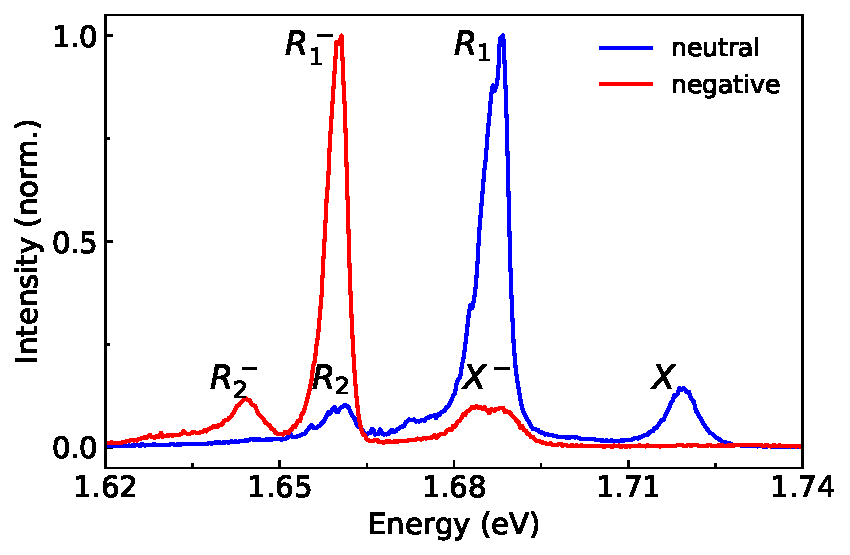
\includegraphics[height=0.65\textwidth]{spectrum_neutral_negative}
	\end{subfigure}
	\begin{subfigure}{0.49\textwidth}
		\caption{}
		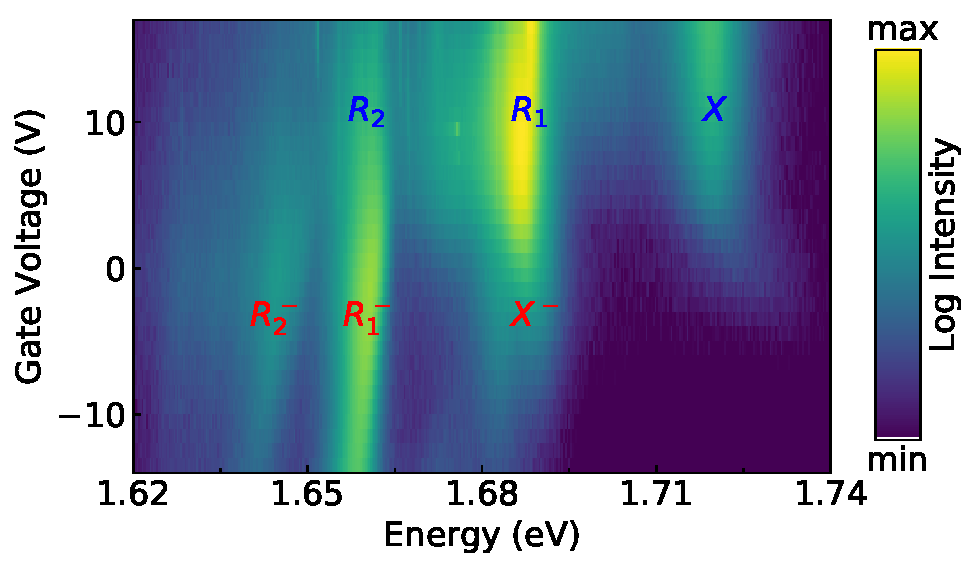
\includegraphics[height=0.65\textwidth]{Voltsweep}
	\end{subfigure}
	\caption{Photoluminescence of \wse at different doping levels. \textbf{A} Spectra in the neutral and negatively charged regime. The \pl of the exciton (X) is clearly visible at the blue end of the spectrum. The replica peaks (R$_1$, R$_2$) correspond to phonon sidebands of momentum indirect excitons. In a negtively charged regime, they vanish in favor of redshifted peaks, that correspond to the trion (X$^-$) with its carracteristic splitting and its momentum indirect counterparts. \textbf{B} Spectral features in a gate-sweep. The plot can be devided into a neutral and charged regime below and above 5V. This threshold is a signature of unintentional n-doping and varies across the sample.}\label{plspectrum}
\end{figure}

\begin{figure}[h]
	\begin{subfigure}{0.49\textwidth}
		\caption{}
		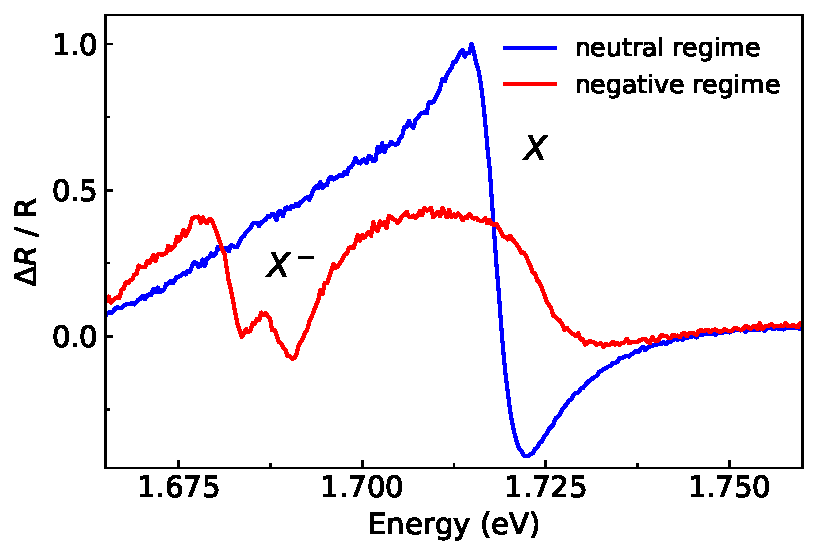
\includegraphics[height=0.65\textwidth]{RF_neut_neg_pure}
	\end{subfigure}
	\begin{subfigure}{0.49\textwidth}
		\caption{}
		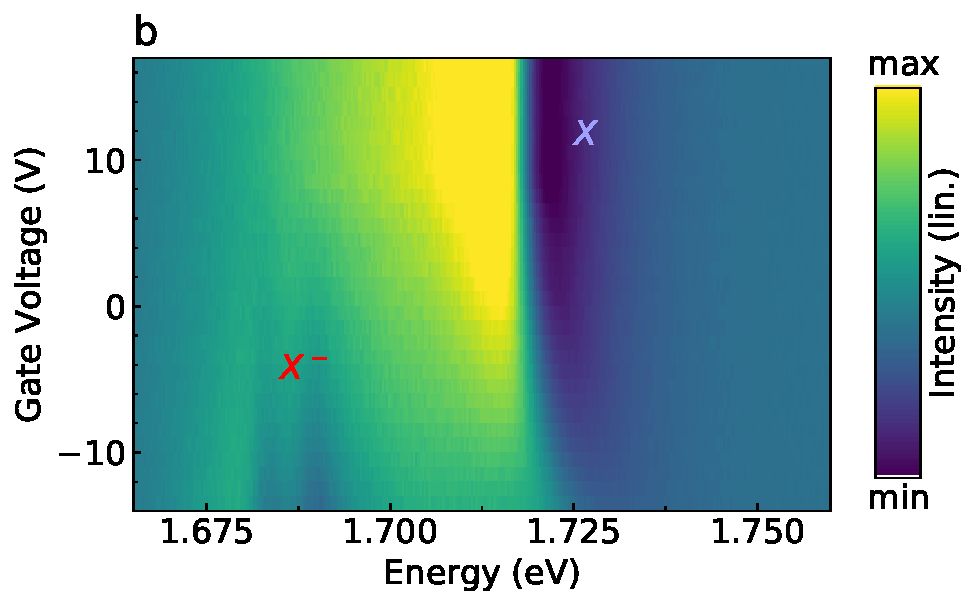
\includegraphics[height=0.65\textwidth]{RF_Voltsweep}
	\end{subfigure}
	\caption{Reflection of \wse at different doping levels. \textbf{A} The reflection spectrum of \wse in a neutral and negatively charged regime. The neutral spectrum shows a strong response, corresponding to the main exciton resonance (X). The absorption of the exciton almost vanishes in the charged spectrum and a double dip appears, that corresponds to the trion resonance, resolving the typical exchange splitting (X$^-$). \textbf{B} Reflection spectra at different voltages. The exciton absorption shows a similar response as in \pl, however stretched to lower voltages. The absorption at the trion resonance can be resolved much better, than the corresponding peaks in \pl. }\label{frspectrum}
\end{figure}

\subsection{Modelling peak shapes}

\begin{figure}[h]
	\begin{subfigure}{0.49\textwidth}
		\caption{}
		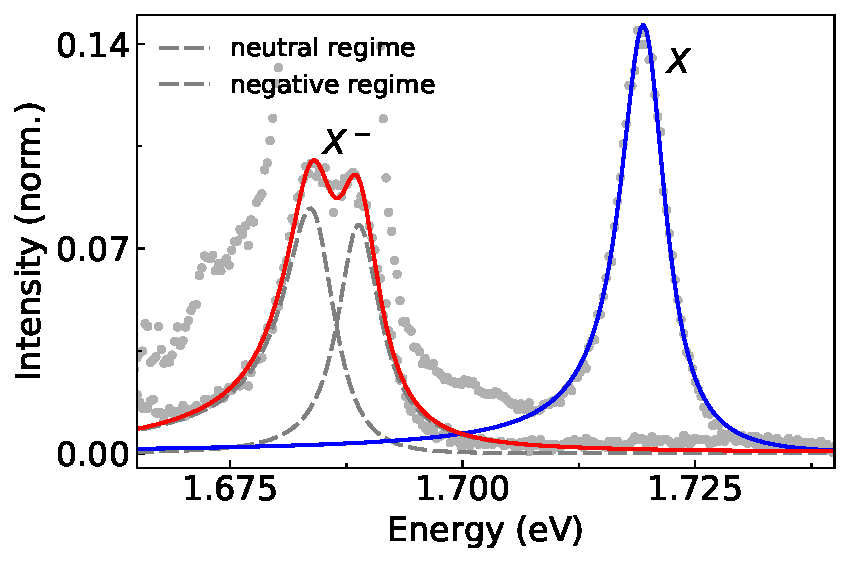
\includegraphics[height=0.65\textwidth]{X_Trion_fit}
	\end{subfigure}
	\begin{subfigure}{0.49\textwidth}
		\caption{}
		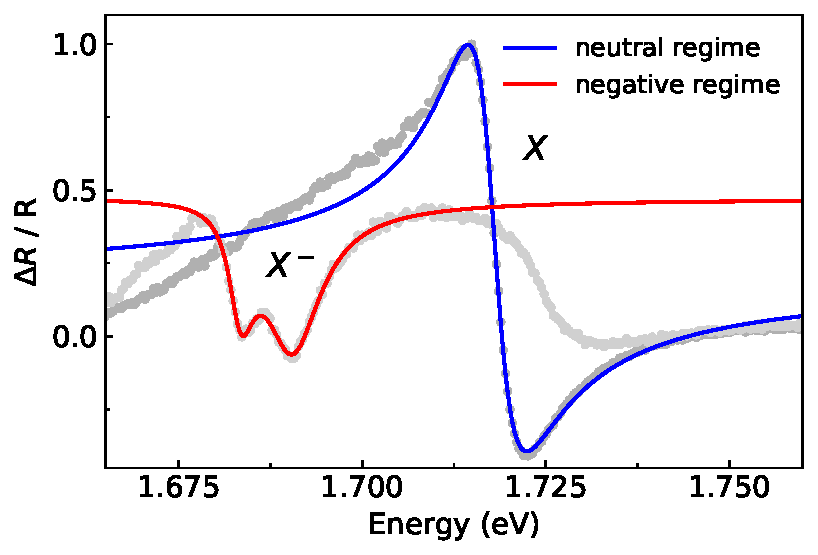
\includegraphics[height=0.65\textwidth]{RF_neut_neg}
	\end{subfigure}
	\caption{Fits of the exciton (X) and trion (X$^-$) features in a neutral and negatively charged spectrum. \textbf{A} \pl : The lineshape in the fitting model is a lorentzian with adaptive linewidth to model the slight asymmetry of the peaks. It is tuned with a sigmoid function, according to a symmetry parameter. The double-peak of the trion feature is a sum of two asymmetric lorentzians. \textbf{B} Reflection: The exciton resonance in this \hbng encapsulated sample does not show a clean dip and can be approximated by a model function corresponding to the scattering cross section of a fano resonance. The trion double dip can be fitted using a sum of two asymmetric lorentzians. However, in contrast to the \pl fit, a constant shifting parameter is added, and the starting values for the scaling parameter are chosen negative.}\label{fits}
\end{figure}

To precisely quantify positions and linewidths of the spectral features, they have to be modelled using appropriate fitting functions. In \pl all peaks should ideally have a lorentzian line shape (see Figure \ref{plspectrum} \textbf{A}). 
\begin{align}
i(\nu)&= \frac{a}{1+\epsilon^2} \\
\epsilon &= \frac{\nu_0 - \nu}{\gamma /2}\label{lorentz}
\end{align}
where $I$ is the intensity, \epsilon is the reduced energy, composed of the energy $\nu$, the peak position $\nu_0$ the linewidth $\gamma$ at \textsc{fwhm}. For a maximum value $a$ of 1, the function is normalized. In the crowded spectrum of an imperfect sample however, this is only an approximation, as the different peaks blend together and can have fine structures, that cannot be resolved as individual features. This leads not only to a broadening of the lines, but also skews the line shape, mostly resulting in a ``red shoulder'' -- higher intensity towards the low-energy end of the peak. To accurately model these features and get good estimates for peak positions as well as linewidths the lorentzian has to be expanded. A generic way of modelling an asymmetric line, that is close to the ``natural'' linewidth is using a lorentzian with variable linewidth $\gamma$, meaning the static linewidth of in \ref{lorentz} is replaced by a smooth sigmoid function, that includes an additional symmetry parameter\cite{stancik_simple_2008}.
\begin{equation} \gamma = \frac{2\gamma_0}{1+e^{k(\nu-\nu_0)}}\label{asymlorentz} \end{equation}
This value is then insterted into \eqref{lorentz}. The symmetry parameter $k$ scales the steepness of the s-cuve sigmoid function and thus the skeewedness of the lineshape. The $\gamma_0$ parameter is identical to $\gamma$ at $\nu_0$ and corresponds to the peaks linewidth. For $k=0$ \eqref{lorentz} collapses to unity and the standard lorentz lineshape is recovered. The asymmetric lorentzian can be used to model all peaks in the \pl spectrum.

In reflection spectroscopy, the signal should correspond to the absorption of the sample. Therefore the straight foreward way to model features would base on a lorentzian function as well, only with a negative sign\footnote{The sign of the fitting functions depends on the definition of the spectrum itself. In this work, the background is substracted from the signal, yielding the reflection off the flake. A flipped sign on the other hand corresponds to the absorption.}. However, the real reflection spectrum is more complicated due to multiple possible effects, not covered by this thesis (see Figure \ref{rfspectrum}). The trion signal in the charged spectrum shows a double dip. This can be modelled by simply adding two negative asymmetric lorentzians and compensating for the positive offset with an additional constant parameter simply added to the function. The main exciton resonance however has a highly asymmetric lineshape, that cannot be modelled with a bare lorentzian (either \eqref{lorentz} or \eqref{asymlorentz}). A more general function is a so called fano resonace. The physical background is the interference between a resonance and a continuous background(referenz fano paper/wiki). 
\begin{equation}
\frac{(q+\epsilon)^2}{(1+\epsilon^2)} = 1 + \frac{q^2+2q\epsilon-1}{1+\epsilon^2}\label{fano}
\end{equation}
where $q$ is the so-called fano parameter. This can be seen as a more general form of \eqref{lorentz}. For $q=0$ the shape of \eqref{fano} reduces to a downwards facing lorentzian. Just like for the trion and all \pl features, the linewidth parameter for \eqref{asymlorentz} can be deployed to skew the function to better fit real data.
Examples of the fitting process for reflection and \pl spectra can be seen in figure \ref{fits}. To use the explained fitting functions, the data was sliced to isolate and fit each feature. 

Besides quantifying the sample quality via the linewidth parameter, the described fitting procedures were extensively used in the next section to find peak positions at different doping levels and different magnetic fields.

\subsection{Measuring the valley zeeman effect at different doping levels}

A functioning gate-tunable device is an ideal base to study different features of \tmds in different doping regimes. The narrow linewidths of clean, \hbng encapsulated \wse samples also allows for the precise quantification of the valley zeeman effect (see theory section), acting on the different states, that make up the \pl and reflection spectra. Using the fitting procedures of the previous section, all features can be quantified in terms of position, linewidth and intensity.

The data, discussed in this section consists of \pl and reflection spectra, that are recorded on a grid of magnetic field between -8 and 8 T, against gate voltage between -15 and 15 V . In this way, every spectral feature can be tracked through a gate sweep, while measuring its g-factor.

\begin{figure}[h]
	\begin{subfigure}{0.32\textwidth}
		\caption{}
		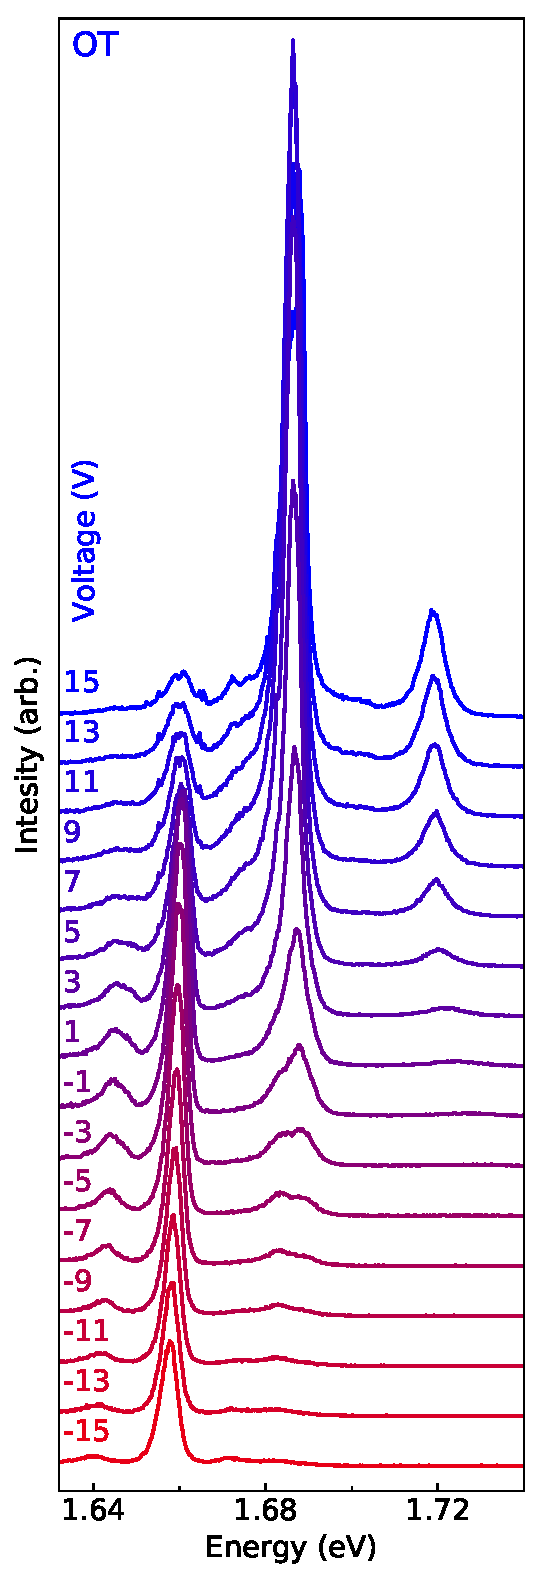
\includegraphics[width=\textwidth]{waterfall_0T}
	\end{subfigure}
	\begin{subfigure}{0.32\textwidth}
		\caption{}
		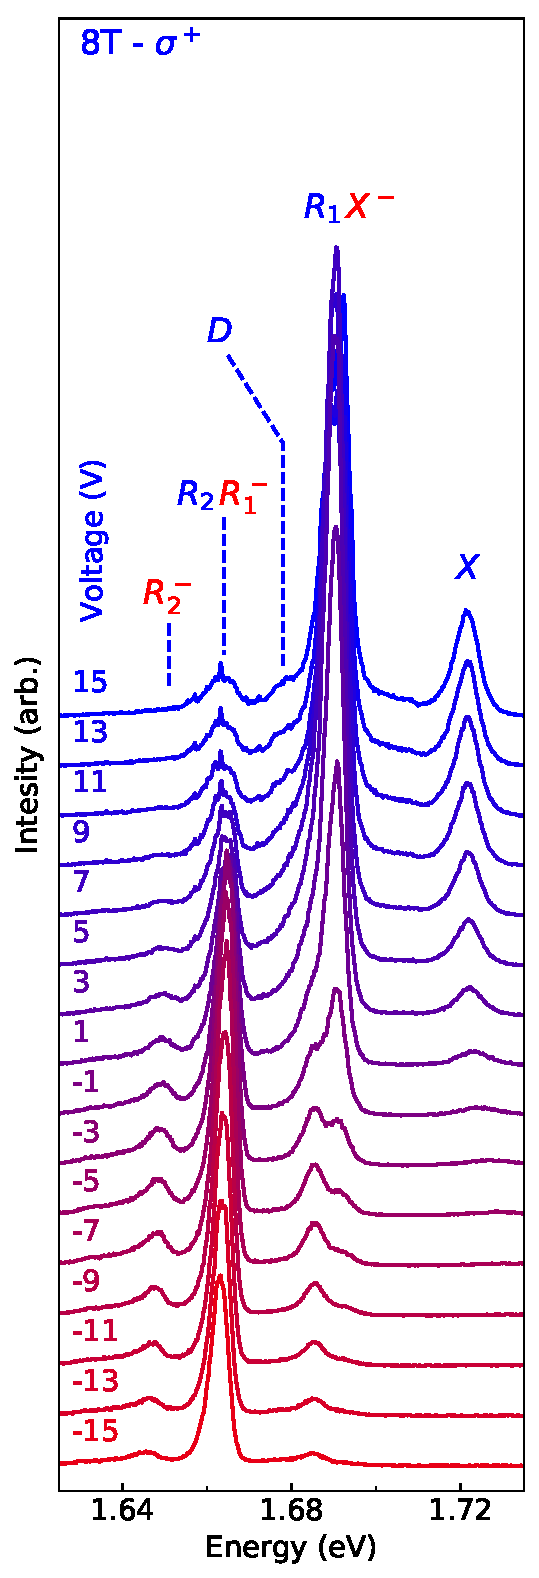
\includegraphics[width=\textwidth]{waterfall_8T_sp}
	\end{subfigure}
	\begin{subfigure}{0.32\textwidth}
		\caption{}
		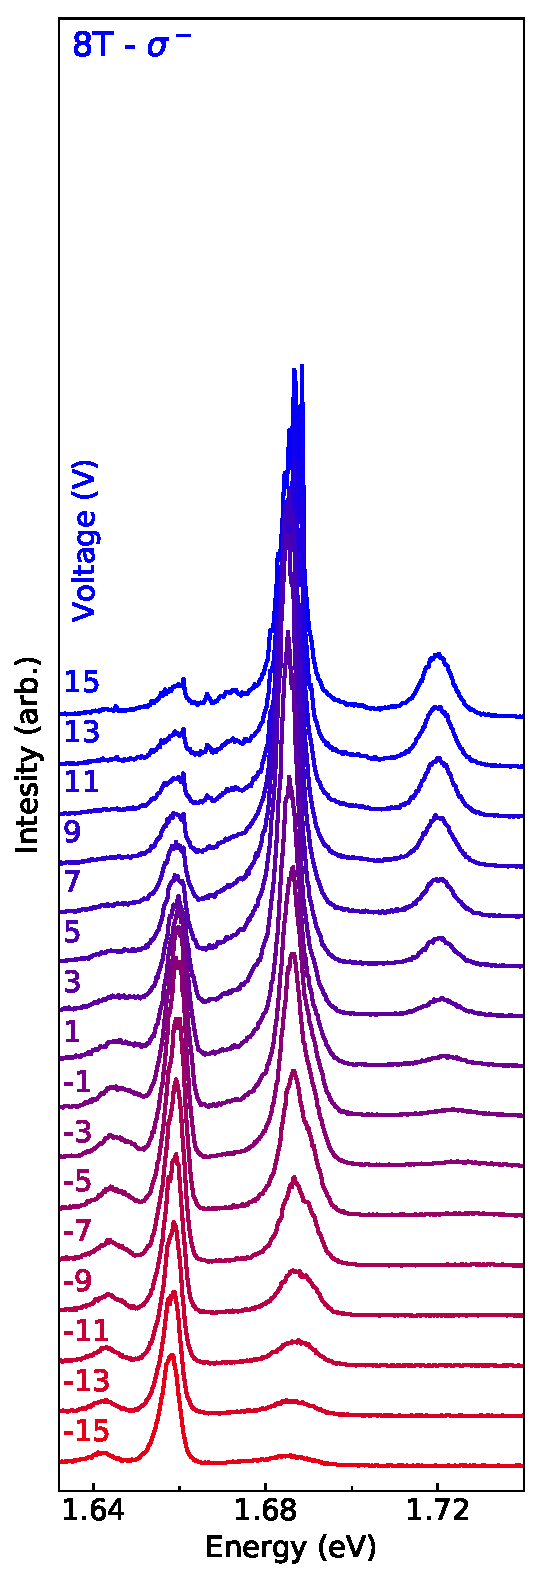
\includegraphics[width=\textwidth]{waterfall_8T_sm}
	\end{subfigure}
	\caption{\textbf{A}  \textbf{B}}\label{waterfall}
\end{figure}

